\documentclass{../indiv}
\graphicspath{{../../images/part2/ch1/}}
\setcounter{chapter}{0}

\begin{document}
	\chapter{寫出你的第一份 \LaTeX 文件 !}
	
	\section{Hello, World! in \LaTeX}
	首先,請大家先進入到Texmaker中新建一份文件(預設快速鍵:\Ctrl+\keystroke{N}),並在畫面中間的原始碼區輸入以下的範例:
	\begin{latexex2}{``Hello, World!" in \LaTeX}{ex:Hello, World!}
\documentclass{article}
\begin{document}
	Hello World! This is a simple example to demonstrate \LaTeX , with no packages used.
\end{document}\end{latexex2}
	輸入完成後存檔(預設快速鍵:\Ctrl + \keystroke{S}),接著就可按下上方工具列的「快速編譯」(預設快速鍵:\keystroke{F1}),讓Texmaker自動呼叫我們先前設定的編譯器。編譯完成後,右側的內建PDF檢視器就會顯示編譯後的PDF檔,我們就不用自己打開Acrobat Reader在那邊慢慢比對,而這也是使用Texmaker的一大好處。整個畫面大概看起來像這樣:
	
	\begin{figure}[H]
		\centering
		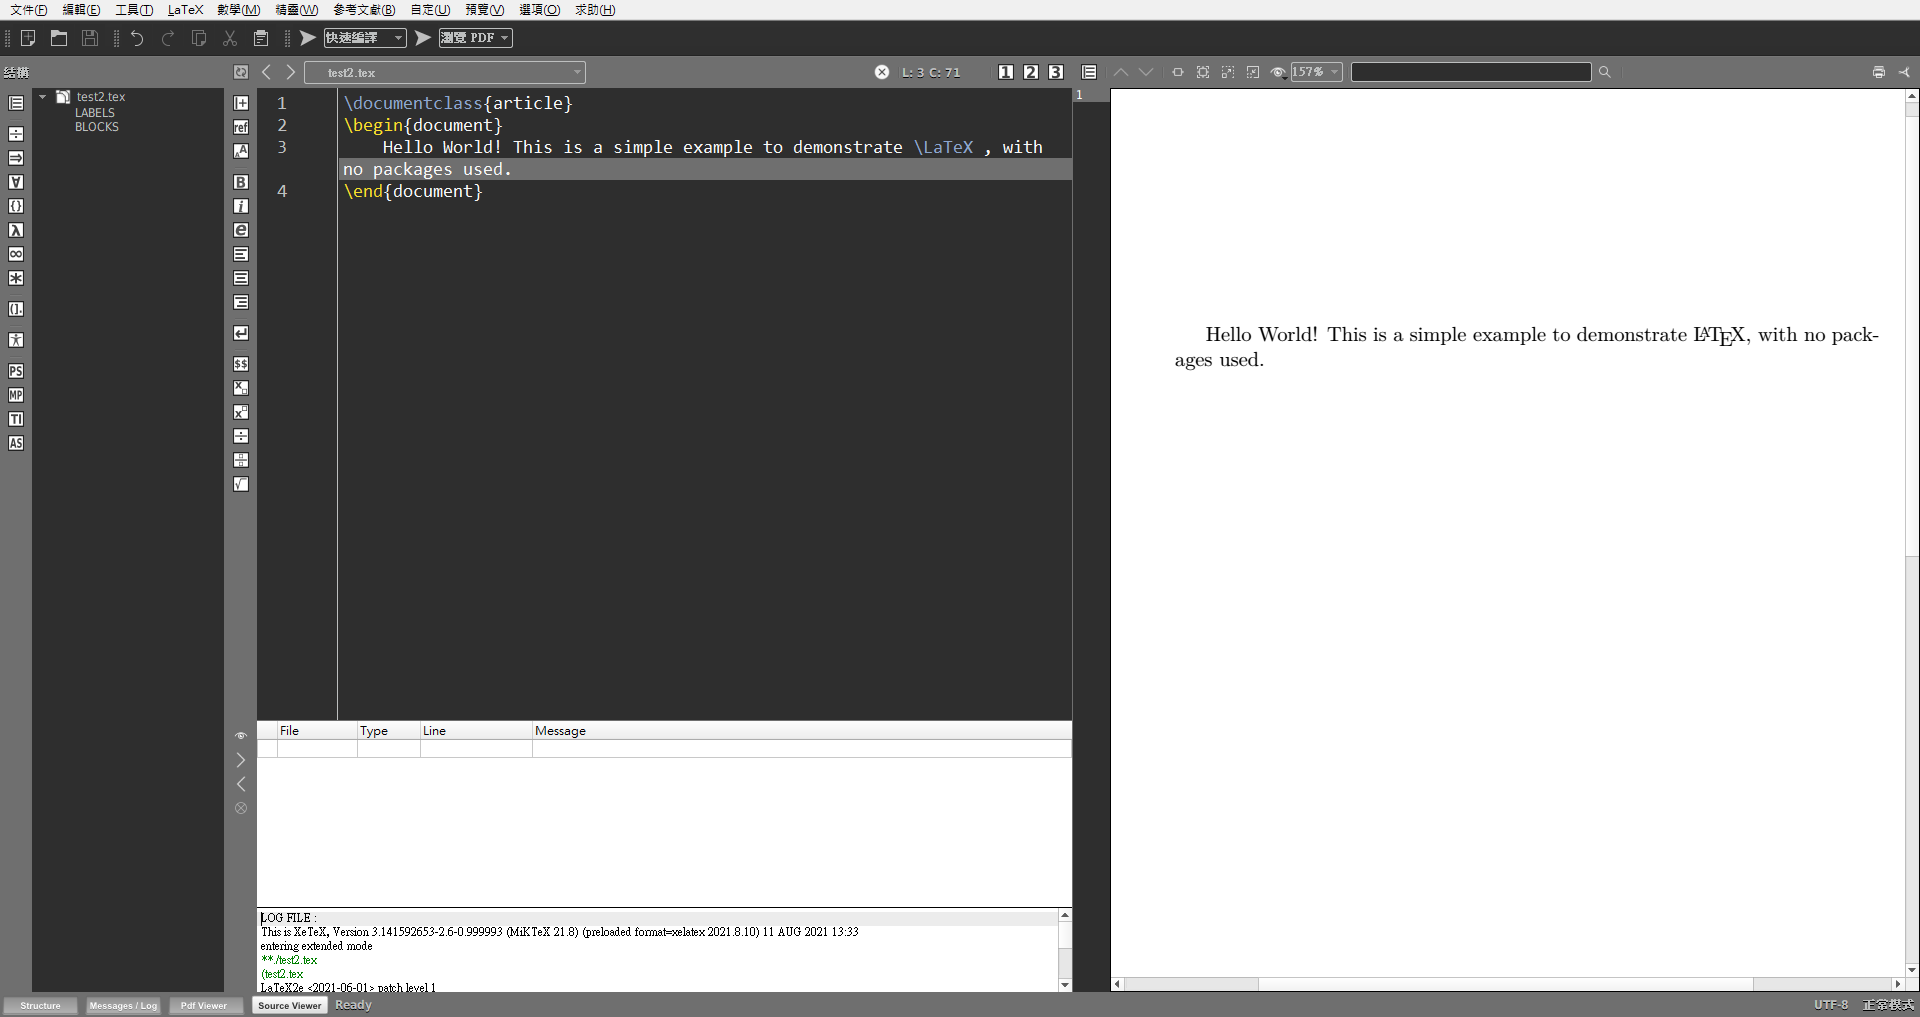
\includegraphics[width=0.7\linewidth]{texmaker-ex1.1-demo.png}
		\caption{完成快速編譯的Texmaker}
	\end{figure}
	\pagebreak
	這份短短4行的文件就可以告訴我們每個\LaTeX 文件都必備的兩個主要架構:出現在\mintinline{LaTeX}{\begin{document}}前的所有東西都稱為「導言」(Preamble);緊接著則是在\mintinline{LaTeX}{\begin{document}}與\mintinline{LaTeX}{\end{document}}之間的「內文」(身體,body)。
	
	導言區的東西不會顯示在最後輸出的文件中,所以這裡通常會包含整份文件的格式設定、引入一些套件或是定義一些指令。在前一頁的範例~\ref{ex:Hello, World!}中,導言就只有簡短的一行而已;但實際上,大型文件的導言動輒上百行都是很可能發生的事。
	
	內文當然就是輸入我們要呈現的內容啦!除了輸入平常的文字以外,我們也可以用\LaTeX 內建的、套件提供的或甚至自己定義的指令,來弄出更炫炮的東西或達到特定的排版效果。
	
	值得注意的是,\LaTeX 在特定的情況中,會主動忽略所有原始碼中的空格與定位字元(Tab),而是用自己的算法找出最佳的分段、分行點與字元間距。在前一頁的範例~\ref{ex:Hello, World!}中,我們就可以看到\LaTeX 自動把第一行縮排,並且在最後一個字``packages"被換行分開時自動補上一個連字號(-)。如果想要違反這些自動的功能,就一定要透過指令來手動調整版面。
	
	此時眼尖的你們應該都發現了,所有\LaTeX 中的指令都是由反除號(\texttt{\textbackslash})開始的。其中,由\mintinline{LaTeX}{\begin{...}}與\mintinline{LaTeX}{\end{...}}包裝起來的又稱為「環境」(Environment)。換言之,先前看到的\texttt{document}環境就是在告訴\LaTeX :這裡面的東西都是要輸出給人看的內容。
	




\end{document}